\section{Résultats et interprétations}

\begin{figure}
  \begin{center}
    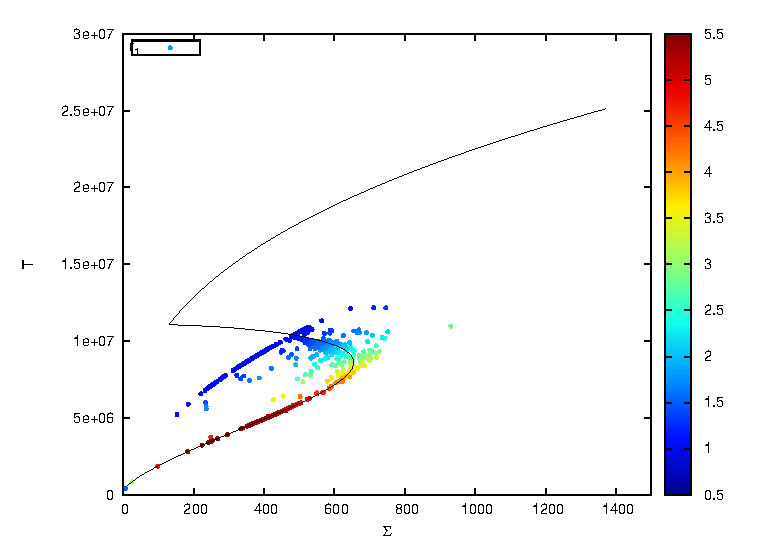
\includegraphics[]{c1.eps}
  \end{center}
  \caption{$T=f(\Sigma)$, $\Delta t = 26141802 s$ (durée de la simulation) pour $r_{1}$. Le gradiant de couleur représente les valeurs de $\tau_{ff}$}
  \label{fig:c1.eps}
\end{figure} 

\begin{figure}
  \begin{center}
    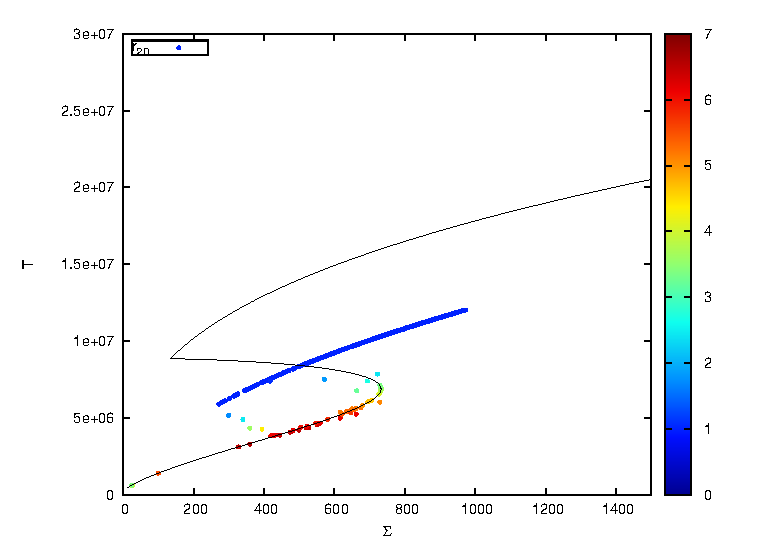
\includegraphics[]{c20.eps}
  \end{center}
  \caption{$T=f(\Sigma)$, $\Delta t = 26141802 s$ (durée de la simulation) pour $r_{20}$. Le gradiant de couleur représente les valeurs de $\tau_{ff}$}
  \label{fig:c20.eps}
\end{figure} 